\documentclass[aspectratio=169]{beamer}
\usetheme{Madrid}
\usecolortheme{whale}

% Additional packages
\usepackage{amsmath, amssymb}
\usepackage{graphicx}
\usepackage{verbatim}
\usepackage{xcolor}
\usepackage{booktabs}

% Create Section Divider Slides
\AtBeginSection[]{
  \begin{frame}
  \vfill
  \centering
  \begin{beamercolorbox}[sep=8pt,center,shadow=true,rounded=true]{title}
    \usebeamerfont{title}\insertsectionhead\par%
  \end{beamercolorbox}
  \vfill
  \end{frame}
}

% Custom colors
\definecolor{myblue}{RGB}{0,82,155}
\setbeamercolor{structure}{fg=myblue}
\setbeamercolor{block title}{bg=myblue!20, fg=myblue}
\setbeamercolor{block body}{bg=myblue!5}

% Frame numbers
\setbeamertemplate{footline}[frame number]

% Navigation symbols
\setbeamertemplate{navigation symbols}{}

% Title and author placeholders
\title{AI-Integrated Washing Machine}
\subtitle{Mini Project Presentation}
\author{
  Mihal Palakkal \quad Ruvais P \quad Mohamed Jaseeb P J \\
  Sajad Hussain Malla \quad Rishap Raj Chaudhary
}
\institute{Department of Computer Science and Engineering \\ \textbf{Cochin University of Science and Technology} \\[0.4cm] 
\textbf{Project Guide:} Ms. Amrutha S Nair \\ \textbf{Project Coordinator:} Dr. Sheena S}
\date{\today}

\begin{document}

% ----------------------------------------------------------------------
% Title Slide
% ----------------------------------------------------------------------
\begin{frame}
\titlepage
\end{frame}

% ----------------------------------------------------------------------
% Outline Slide (optional, but professional)
% ----------------------------------------------------------------------
\begin{frame}{Outline}
\tableofcontents
\end{frame}

% ======================================================================
% Section: Introduction
% ======================================================================
\section{Introduction}

% ----------------------------------------------------------------------
% Slide 2: Problem Statement & Objective
% ----------------------------------------------------------------------
\begin{frame}{Problem Statement \& Objective}
\begin{itemize}
    \item \textbf{Problem:} Existing semi-automatic machines waste water, detergent, and often damage clothes due to fixed wash cycles.
    \item \textbf{Objective:} Convert a semi-automatic washing machine into a fully automated, AI-powered system that:
    \begin{itemize}
        \item Identifies cloth type (fabric, fiber category, soil level) using a smartphone camera.
        \item Optimizes wash parameters (detergent, water level, spin time, temperature, mechanical action) to extend cloth lifetime.
    \end{itemize}
\end{itemize}
\vspace{0.5cm}
\centering
\alert{Goal:} \emph{Intelligent washing that preserves fabric quality and conserves resources.}
\end{frame}

% ----------------------------------------------------------------------
% Slide 3: System Overview (Architecture Diagram)
% ----------------------------------------------------------------------
\begin{frame}{System Overview}
\frametitle{System Architecture}
\begin{center}
\begin{minipage}{0.9\textwidth}
\centering
\textbf{Cloth Image} $\rightarrow$ \textbf{Mobile App} $\rightarrow$ \textbf{Gemini API} $\rightarrow$ \textbf{Arduino} $\rightarrow$ \textbf{Washing Machine}
\end{minipage}
\end{center}

\vspace{0.5cm}
\textbf{Two-Stage AI Pipeline:}
\begin{enumerate}
    \item \textbf{Fabric Detection} – Identifies fabric type, fiber category, and soil level.
    \item \textbf{Wash Parameter Calculation} – Computes optimal wash settings based on Stage 1 output.
\end{enumerate}

\end{frame}

\begin{frame}{System Architecture Overview}
\centering
\vspace{0.2cm}
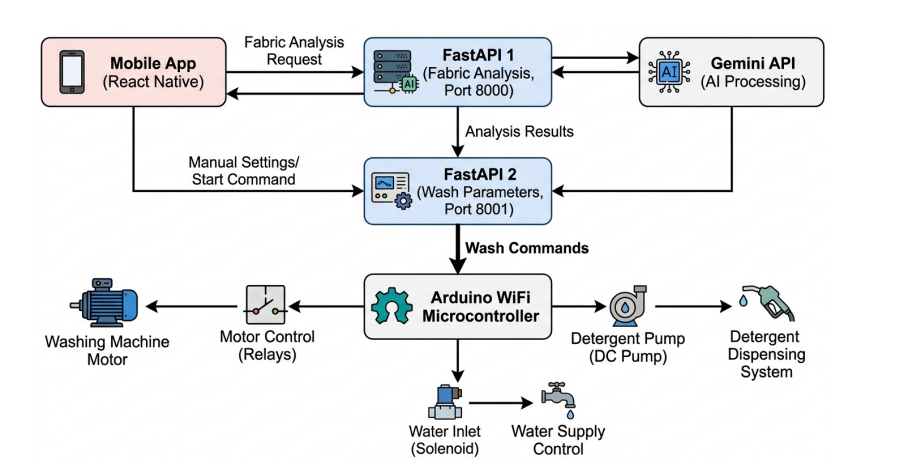
\includegraphics[width=0.9\textwidth, height=0.65\textheight, keepaspectratio]{img/system_overview.png}
\\[0.4cm]{\normalsize Flow: Image $\rightarrow$ Gemini (Stage 1 \& 2) $\rightarrow$ Arduino $\rightarrow$ Machine Actuation}
\end{frame}

% ======================================================================
% Section: Hardware Design
% ======================================================================
\section{Hardware Design}

% ----------------------------------------------------------------------
% Slide 4: Hardware Components (two columns)
% ----------------------------------------------------------------------
\begin{frame}{Hardware Components}
\begin{columns}[T]
\begin{column}{0.48\textwidth}
\begin{block}{Core \& Commutation}
\begin{itemize}
    \item Semi-automatic Washing Machine
    \item Arduino WiFi R4
    \item 3-Phase Motor (240V, 10A)
    \item 2 Rotation Relays + 1 Solenoid Relay
\end{itemize}
\end{block}
\end{column}
\begin{column}{0.48\textwidth}
\begin{block}{Dispensing \& Actuation}
\begin{itemize}
    \item Solenoid Water Inlet Valve
    \item 5V DC Water Pump (Detergent)
    \item Transistor TAS122
    \item 12V L298N DC Motor Driver
\end{itemize}
\end{block}
\end{column}
\end{columns}
\vspace{0.3cm}
\centering
\small All components integrated to automate washing, dispensing, and motor control.
\end{frame}

% ----------------------------------------------------------------------
% Slide 5: Hardware Design & Control Logic
% ----------------------------------------------------------------------
\begin{frame}{Hardware Design \& Control Logic}
\begin{itemize}
    \item \textbf{Motor Control:} Clockwise 5s $\rightarrow$ Stop 2s $\rightarrow$ Counter-clockwise 5s (loop) using relays.
    \item \textbf{Detergent Dispenser:} Linear regression model calculates valve open time.
    \begin{itemize}
        \item Data collected: volume dispensed at 50~ms, 100~ms, \dots, 2400~ms intervals.
        \item Linear regression equation implemented in Arduino code for precise dispensing.
    \end{itemize}
    \item \textbf{Water Inlet Valve:} Same calibration approach ensures accurate water filling.
\end{itemize}
\vspace{0.3cm}
\begin{block}{Linear Regression Example}
\[
\text{Open Time (ms)} = a \times \text{Desired Volume (ml)} + b
\]
\small (coefficients $a,b$ obtained from experimental calibration)
\end{block}
\end{frame}

% ----------------------------------------------------------------------
% Slide 6: Detergent Dispenser Calibration
% ----------------------------------------------------------------------
\begin{frame}{Detergent Dispenser Calibration}
\begin{columns}[T]
\begin{column}{0.45\textwidth}
    \begin{block}{Calibration Data}
    \centering
    \resizebox{\textwidth}{!}{
    \begin{tabular}{cc|cc|cc}
        \toprule
        \textbf{Time (ms)} & \textbf{Vol (ml)} & \textbf{Time (ms)} & \textbf{Vol (ml)} & \textbf{Time (ms)} & \textbf{Vol (ml)} \\
        \midrule
        50 & 0.0 & 650 & 10.25 & 1400 & 26.5 \\
        100 & 0.0 & 700 & 11.5 & 1500 & 28.0 \\
        150 & 0.0 & 750 & 12.0 & 1600 & 30.0 \\
        200 & 0.5 & 800 & 13.0 & 1700 & 33.0 \\
        250 & 2.0 & 850 & 15.0 & 1800 & 35.5 \\
        300 & 3.0 & 900 & 16.5 & 1900 & 39.5 \\
        350 & 4.5 & 950 & 18.0 & 2000 & 41.5 \\
        400 & 5.0 & 1000 & 19.0 & 2100 & 44.5 \\
        450 & 6.0 & 1050 & 20.0 & 2200 & 46.0 \\
        500 & 7.5 & 1100 & 21.0 & 2300 & 48.0 \\
        550 & 8.5 & 1200 & 23.0 & 2400 & 50.5 \\
        600 & 9.75 & 1300 & 25.5 & -- & -- \\
        \bottomrule
    \end{tabular}
    }
    \end{block}
\end{column}
\begin{column}{0.55\textwidth}
    \centering
    \begin{block}{Linear Regression Model}
    \centering
    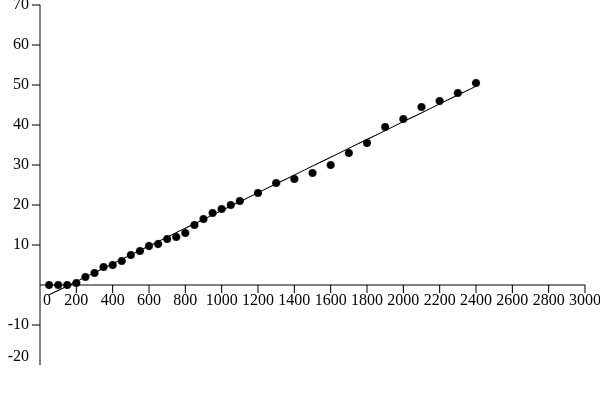
\includegraphics[width=0.9\textwidth, height=0.4\textheight, keepaspectratio]{img/graph.png}\\
    \end{block}
    
    \vspace{0.2cm}
    \resizebox{0.8\textwidth}{!}{
    \begin{tabular}{lc}
        \toprule
        \textbf{Coefficient} & \textbf{Value} \\
        \midrule
        $a$ (slope) & 0.022176 \\
        $b$ (intercept) & -3.569687 \\
        $R^2$ value & 0.997 (approx.) \\
        \bottomrule
    \end{tabular}
    }
    \\[0.1cm]
    {\scriptsize \textbf{Table 5.2:} Linear Regression Coefficients}
\end{column}
\end{columns}
\end{frame}

% ======================================================================
% Section: AI & Backend
% ======================================================================
\section{AI \& Backend}

% ----------------------------------------------------------------------
% Slide 6: Stage 1 – Fabric Analysis (Prompt Engineering)
% ----------------------------------------------------------------------
\begin{frame}[fragile]{AI \& Prompt Engineering – Stage 1}
\frametitle{Fabric Analysis (Gemini API)}
\small
\begin{columns}[T]
\begin{column}{0.5\textwidth}
\textbf{Multi-stage prompt system} extracts:
\begin{itemize}
    \item Fabric name
    \item Fiber category
    \item Soil level (1–5 scale)
\end{itemize}
\vspace{0.2cm}
\textbf{Visual markers analyzed:} \\ diagonal ribbing, fiber luster, fold behavior.
\end{column}
\begin{column}{0.5\textwidth}
\begin{block}{Soil Level Scale}
\footnotesize
\begin{description}
    \item[Level 1:] Clean
    \item[Level 3:] Moderately Dirty
    \item[Level 5:] Emergency
\end{description}
\end{block}
\end{column}
\end{columns}
\end{frame}

\begin{frame}[fragile]{AI \& Prompt Engineering – Stage 1 (Output)}
\frametitle{JSON Output Format}
\begin{block}{Output JSON (Stage 1)}
\begin{verbatim}
{
  "material_type": "cotton twill",
  "fiber_category": "Natural",
  "description": "Heavy cotton fabric with diagonal ribs",
  "dirt_level": 3,
  "confidence_score": 0.92
}
\end{verbatim}
\end{block}
\end{frame}

% ----------------------------------------------------------------------
% Slide 7: Stage 2 – Wash Parameter Calculation
% ----------------------------------------------------------------------
\begin{frame}[fragile]{AI \& Prompt Engineering – Stage 2}
\frametitle{Wash Parameter Calculation}
\small
Takes JSON from Stage 1 and computes optimal wash settings:

\begin{columns}[T]
\begin{column}{0.5\textwidth}
\begin{itemize}
    \item Detergent: baseline 20~ml, adjusted
    \item Soak: 0-30~min
    \item Spin: 3-12~min based on fabric
    \item Water: standard 35~L
\end{itemize}
\end{column}
\begin{column}{0.5\textwidth}
\begin{itemize}
    \item Wash Cycles: (1–2)
    \item Temp: up to 60~°C 
    \item Action: Gentle / Normal / Heavy
\end{itemize}
\end{column}
\end{columns}
\end{frame}

\begin{frame}[fragile]{AI \& Prompt Engineering – Stage 2 (Output)}
\frametitle{Wash Parameters JSON}
\begin{block}{Output JSON (Stage 2)}
\begin{verbatim}
{
  "detergent_ml": 28,
  "soak_minutes": 15,
  "spin_minutes": 8,
  "water_liters": 35,
  "wash_cycles": 2,
  "temperature_c": 45,
  "mechanical_action": "Normal"
}
\end{verbatim}
\end{block}
\end{frame}

% ----------------------------------------------------------------------
% Slide 8: FastAPI Backend (2 APIs)
% ----------------------------------------------------------------------
\begin{frame}{FastAPI Backend}
\textbf{Two independent microservices:}

\vspace{0.2cm}
\begin{columns}[T]
\begin{column}{0.48\textwidth}
\begin{block}{API 1 – Fabric Analysis (Port 8000)}
\small
\begin{itemize}
    \item Input: Cloth image
    \item Uses Pillow + Gemini API
    \item Predicts: fiber type, dirt level, description
    \item \textbf{Human-in-the-Loop} feedback for correcting predictions
\end{itemize}
\end{block}
\end{column}
\begin{column}{0.48\textwidth}
\begin{block}{API 2 – Wash Parameter Calculator}
\small

\end{block}
\end{column}
\end{columns}

\vspace{0.2cm}
\textbf{Tech Stack:} Python, FastAPI, Pydantic, Pillow, Gemini API, OpenAPI
\end{frame}

% ======================================================================
% Section: Mobile App & Testing
% ======================================================================
\section{Mobile App \& Testing}

% ----------------------------------------------------------------------
% Slide 9: Mobile App (React Native Expo)
% ----------------------------------------------------------------------
\begin{frame}{Mobile App (React Native Expo)}
\frametitle{User Interface – Tab-Based Navigation}
\begin{columns}[T]
\begin{column}{0.48\textwidth}
\begin{block}{5 Screens}
\begin{enumerate}
    \item Dashboard
    \item Fabric Analysis
    \item Wash Progress
    \item Manual Override
    \item Settings
\end{enumerate}
\end{block}
\end{column}
\begin{column}{0.48\textwidth}
\begin{block}{Key Features}
\begin{itemize}
    \item Reusable UI components (Step Indicators, Notification Cards)
    \item TypeScript interfaces for data integrity (Fabric, MachineMetrics, CycleState)
    \item Tailwind CSS utility-first styling
    \item Async API service layer connecting to backend
    \item Cross-platform (iOS \& Android)
\end{itemize}
\end{block}
\end{column}
\end{columns}
\vspace{0.3cm}
\centering \small App communicates with FastAPI backends via REST calls.
\end{frame}

\begin{frame}{Mobile App Screenshots (1/2)}
\centering
\vfill
    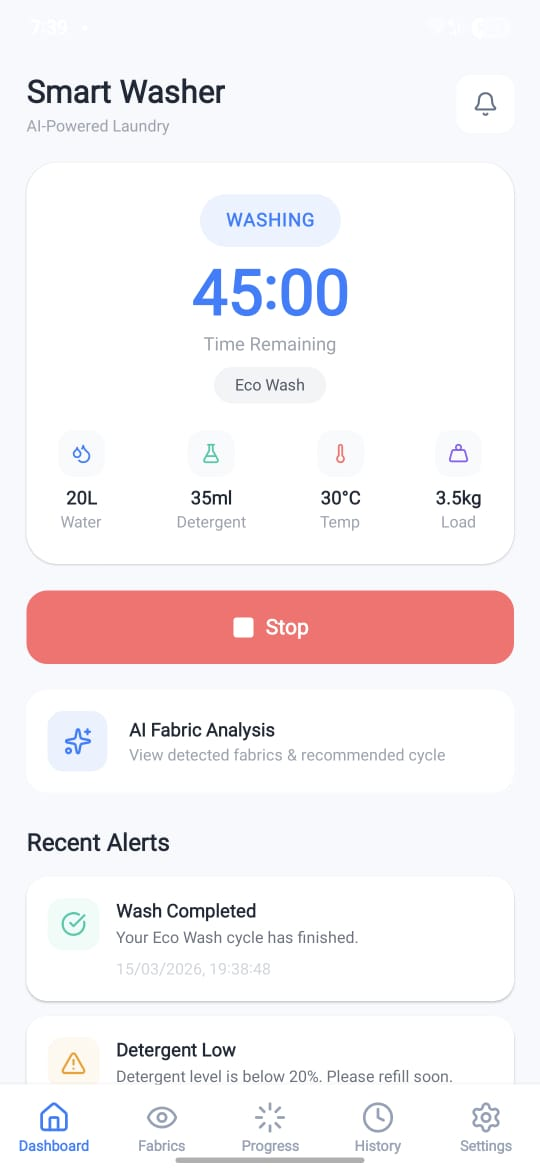
\includegraphics[height=0.65\textheight, keepaspectratio]{img/app1.jpeg}\hfill
    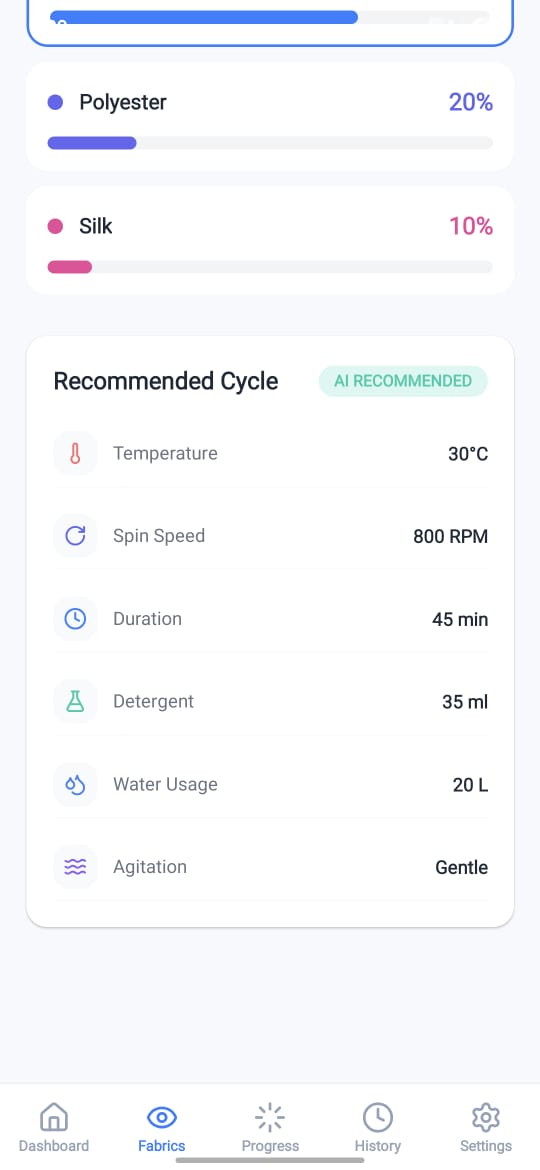
\includegraphics[height=0.65\textheight, keepaspectratio]{img/app2.jpeg}\hfill
    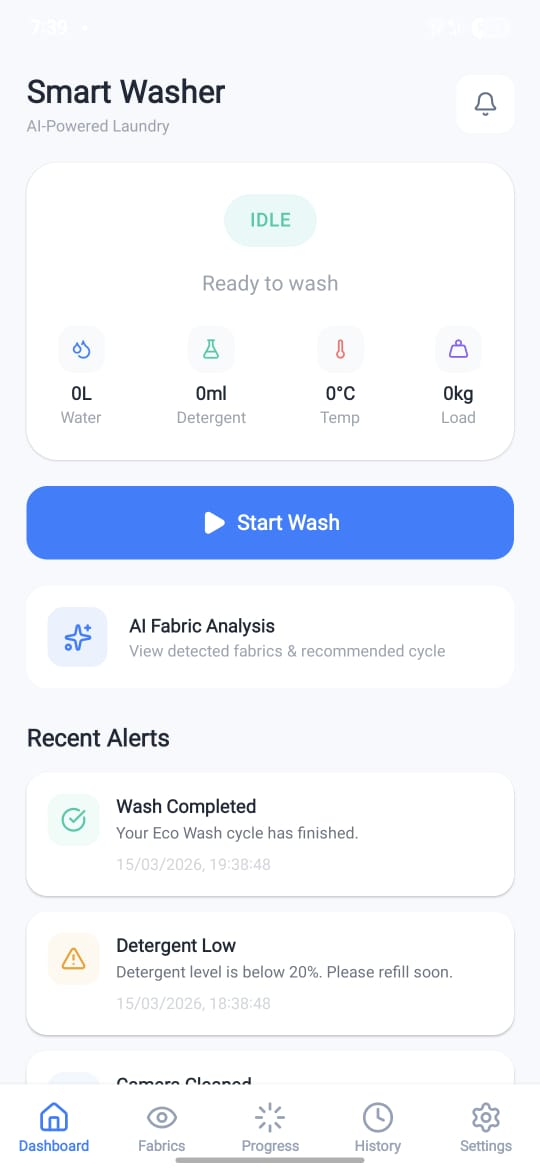
\includegraphics[height=0.65\textheight, keepaspectratio]{img/app3.jpeg}\hfill
    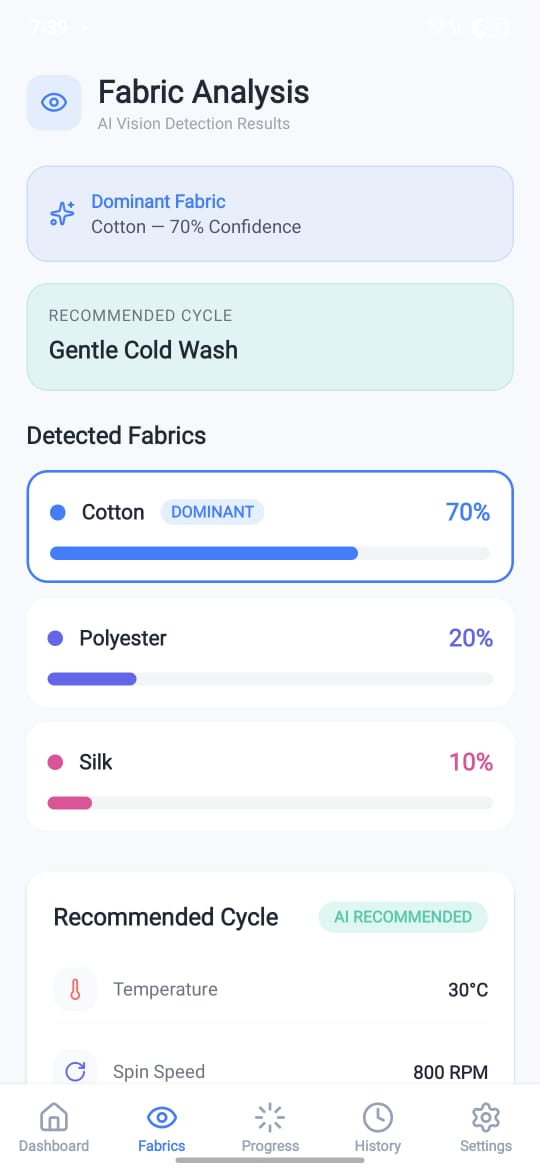
\includegraphics[height=0.65\textheight, keepaspectratio]{img/app4.jpeg}
\vfill
\end{frame}

\begin{frame}{Mobile App Screenshots (2/2)}
\centering
\vfill
    
\includegraphics[height=0.65\textheight, keepaspectratio]{img/app5.jpeg}\hspace{0.5cm}
    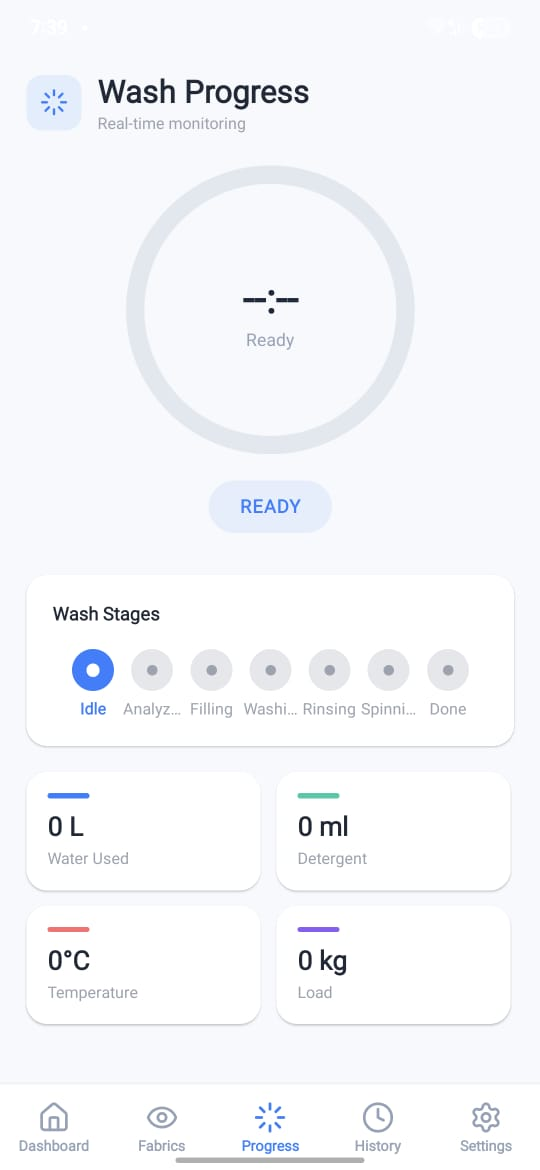
\includegraphics[height=0.65\textheight, keepaspectratio]{img/app6.jpeg}\hspace{0.5cm}
    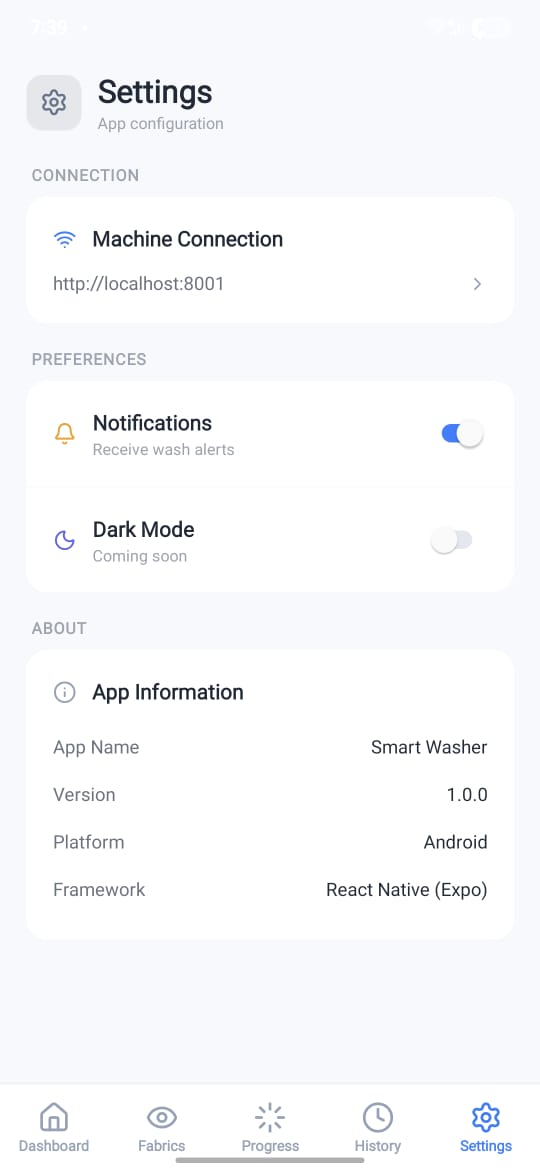
\includegraphics[height=0.65\textheight, keepaspectratio]{img/app7.jpeg}
\vfill
\end{frame}

% ----------------------------------------------------------------------
% Slide 10: Dataset Validation & Testing
% ----------------------------------------------------------------------
\begin{frame}{Dataset Validation \& Testing}
\begin{itemize}
    \item Test cases designed from \textbf{heavy-duty (Denim)} to \textbf{delicate (Chiffon)}.
    \item \textbf{Human-in-the-Loop (HITL)} testing for misclassifications:
    \begin{itemize}
        \item Example: Differentiating \emph{Cotton Twill} vs \emph{Synthetic Blends}
        \item Iterative prompt refinement eliminated identification errors.
    \end{itemize}
    \item Standardized JSON output ensures seamless hardware integration.
    \item Validation of detergent dispensing using linear regression (error $< 5\%$).
\end{itemize}
\vspace{0.3cm}
\begin{exampleblock}{Result}
\centering Reliable classification across 15+ fabric types with high confidence.
\end{exampleblock}
\end{frame}

% ======================================================================
% Section: Results & Future
% ======================================================================
\section{Results \& Future Scope}

% ----------------------------------------------------------------------
% Slide 11: Results & Key Achievements
% ----------------------------------------------------------------------
\begin{frame}{Results \& Key Achievements}
\begin{itemize}
    \item \textbf{Accurate Fabric Classification:} High confidence scores across multiple fabric types.
    \item \textbf{Precise Detergent Dispensing:} Linear regression validated against real measurements.
    \item \textbf{End-to-End Automation:} Image scan $\rightarrow$ AI decision $\rightarrow$ Hardware execution.
    \item \textbf{Increased Cloth Lifetime:} Optimized parameters per fabric type reduce wear and tear.
    \item \textbf{Fully Functional Dual-API System:} With real-time feedback loop for continuous improvement.
\end{itemize}
\vspace{0.3cm}
\begin{exampleblock}{Success}
\centering Successfully converted a semi-automatic machine into an intelligent, adaptive washing system.
\end{exampleblock}
\end{frame}

% ----------------------------------------------------------------------
% Slide 12: Conclusion & Future Scope
% ----------------------------------------------------------------------
\begin{frame}{Conclusion \& Future Scope}
\textbf{Conclusion:}
\begin{itemize}
    \item Demonstrated a low-cost, AI-integrated laundry automation system.
    \item Bridges computer vision, prompt engineering, embedded systems, and mobile development.
\end{itemize}
\vspace{0.3cm}
\textbf{Future Scope:}
\begin{itemize}
    \item Add weight sensor for load-based optimization.
    \item Cloud dashboard for wash history analytics.
    \item Support for multi-cloth batch scanning.
    \item Integration with smart home ecosystems (Google Home, Alexa).
\end{itemize}
\end{frame}

% ----------------------------------------------------------------------
% Thank You / Q&A Slide
% ----------------------------------------------------------------------
\begin{frame}{Thank You}
\begin{center}
\Huge Thank You! \\[1cm]
\Large Questions? \\[0.5cm]
\small \emph{We welcome your feedback.}
\end{center}
\end{frame}

\end{document}